\chapter{Backpropagation}\label{ch:backpropagation}
\label{sec:backpropagation}

Simple learning can be achieved by expressing the unknown parameters of a problem in a cost function and then following its gradient to minimize cost. This is straightforward if the cost function is directly differentiable.Calculating the partial derivatives for the error function manually is not straightforward in a multi-layer neural network (Chapter \ref{chap:ann}), however, which is a computation graph that transforms the input $x$ by a series of multiplications and non-linear activation functions, which in turn require the chain rule.

Applying the chain rule can be done in two ways: moving forwards or backwards through the computation graph. Actually doing this by hand for a simple graph shows that going backwards is significantly more efficient. Manually deriving the individual partial derivatives also illustrates that many of the computations can actually be recycled. This solution is known as \index{Backpropagation}\textsl{backpropagation} \cite{rumelhart1985learning}, a technique that has been independently discovered in multiple fields. The derivation below follows \cite{backpropagation}. Note, that we are using the notation from Chapter \ref{chap:ann}) and Section \ref{sec:lossfunction} in particular. 

In a first step, we note that the error function is a sum over all input-output pairs:
\begin{equation}
\frac{\partial E(x,y,w)}{\partial w_{i,j}^k}=\frac{1}{2N}\sum^N_{d=1}\frac{\partial}{\partial w_{i,j}^k}(\hat{y_d}-y_d)^2=\frac{1}{2N}\sum_{d=1}^N\frac{\partial E_d}{\partial w_{i,j}^k}
\end{equation}
We will therefore focus on only one input-output pair $(x_d,y_d)$ and differentiate against $w_{i,j}^k$. (The index $d$ has been chosen to avoid confusion with the indices $i$ and $j$, and will be omitted for brevity in the remainder).

\paragraph{The Chain rule} The key for understanding the backpropagation algorithm is to apply the chain rule in a correct way. Specifically, if a variable $z$ depends on the variable $y$, which itself depends on the variable $x$, then
\begin{equation}
\frac{dz}{dx}=\frac{dz}{dy}\frac{dy}{dx}
\end{equation}

With the output layer having index $m$ and a single output ($a^m_1$), the error is computed by the recursive formula
\begin{equation}
E(x,y,w_{i,j})=\frac{1}{2}(\hat{y}-y)^2=\frac{1}{2}(g(a_1^m)-y)^2=
\frac{1}{2}\left(g\left(\sum_{l=0}^{r_{m-1}}w_{l,1}^mo_l^{m-1}\right)-y\right)^2.
\end{equation}
We observe that the variable $E$ depends on the outputs $o_l^{m-1}$ with $l=0..r_{m-1}$ from the previous layer. Recall that $o_l^{m-1}$ is simply the activation $a_l^{m-1}$ after applying the activation function. Also recall that $w^m_{i,1}$ are weights coming into node $1$. The error with respect to $w_{i,j}$ is therefore dependent on all $a^k_j$ for all previous layers. This is also visualized in \cref{fig:backpropnotation3}.

\begin{figure}[htb]
    \centering
    % 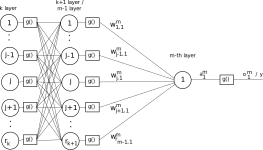
\includegraphics[width=0.8\columnwidth]{figs/backpropnotation3}
    \def\svgwidth{\textwidth}
    \import{./figs/}{backpropnotation3.pdf_tex}
    \caption{Last three layers of a neural network with a single output neuron, illustrating dependencies between function values and the output when moving along the computation graph backwards.\label{fig:backpropnotation3}}
\end{figure}

The chain rule therefore states
\begin{equation}
\frac{\partial E}{\partial w_{i,j}^k}=\frac{\partial E}{\partial a_i^k}\frac{\partial a_i^k}{\partial w_{i,j}^k}
\end{equation}

\paragraph{Error at layer k}
The first term is part of a vector called the ``error at layer $k$''  that consists of errors at all nodes $j$ in layer $k$ and is denoted by
\begin{equation}
\delta^k_j=\frac{\partial E}{\partial a_j^k}
\end{equation}

The second term can be computed from the definition of $a_j^k$ above
\begin{equation}
\frac{\partial a^k_j}{\partial w_{i,j}^k}=\frac{\partial}{\partial w_{i,j}^k}\left(\sum_{l=0}^{r_{k-1}} w_{l,j}^k o^{k-1}_l\right)=o^{k-1}_i
\end{equation}
which follows from the fact that only the term involving $o^{k-1}_i$ is the one where $l=i$. In case you expect the chain rule to apply further, remember that $o^{k-1}_i$ is actually not dependent on $w_{i,j}^k$, so you are done here.

Thus, the partial derivative of the error function $E$ with respect to weight $w_{i,j}^k$ is
\begin{equation}
\frac{\partial E}{\partial w^k_{i,j}}=\delta^k_jo^{k-1}_i.
\end{equation}

We can see that the error $E$ with respect to each individual weight $w_{i,j}^k$ in a layer $k$ depends on the output of the layers coming before that. This is intuitive, as information propagates through the network. We will now also show that the error term $\delta_j^k$ actually depends on the error at layers above $k$, that is stems from the error $\hat{y}-y$ that we ultimately want to minimize.

\section{Backward propagation of error}

In order to show how the error term $\delta^k_i$ relates to the error  at the output layer, we will start working backwards. Let $m$ be the index of the output layer. We are also only considering a network with one output neuron, that is $j=1$. The error at this final layer $m$ is given by
\begin{equation}
E=\frac{1}{2}(\hat{y}-y)^2=\frac{1}{2}(g(a_1^m)-y)^2
\end{equation}
Using the chain rule $\frac{\partial E}{\partial w_{i,1}^m}=\frac{\partial E}{\partial a^m_i}\frac{\partial a^m_i}{\partial w^k_{i,1}}$ as before yields
\begin{equation}
\delta^m_1=\frac{\partial E}{\partial a^m_1}=(g(a^m_1)-y)g'(a^m_1)=(\hat{y}-y)g'(a^m_1)
\end{equation}
for the error at layer $m$ and
\begin{equation}
\frac{\partial a^m_1}{\partial w^k_{i,1}}=o_i^{m-1}.
\end{equation}

Together, these two result into
\begin{equation}
\frac{\partial E}{\partial w_{i,1}^m}=(\hat{y}-y)g'(a^m_1)o_i^{m-1}.
\end{equation}

We continue to use the chain rule to work backward along the computation graph. Specifically, the activation $a^k_j$ at node $j$ in layer $k$, with $1\leq k <m$ feeds into all nodes $l=1..r^{k+1}$ of layer $k+1$. Therefore, the error $\delta^k_j$ calculates to
\begin{equation}
\delta^k_j=\frac{\partial E}{\partial a^k_j}=\sum_{l=1}^{r^{k+1}}\frac{\partial E}{\partial a_l^{k+1}}\frac{\partial a_l^{k+1}}{\partial a^k_j}
\end{equation}

Using $\delta^{k+1}_l=\frac{\partial E}{\partial a_l^{k+1}}$, the above equation simplifies to
\begin{equation}
\delta^k_j=\sum_{l=1}^{r^{k+1}}\delta_l^{k+1}\frac{\partial a_l^{k+1}}{\partial a^k_j}
\end{equation}

Inspecting the computation graph or the definition of $a^k_j$, we recall that $a_l^{k+1}$ receives the output $g(a_j^k)$ from every node $j=1..r^k$ in layer $k$ via weight $w_{j,l}^{k+1}$, i.e.
\begin{equation}
a_l^{k+1}=\sum_{j=1}^{r^k}w_{j,l}^{k+1}g(a_j^k)
\end{equation}
allowing us to compute the partial derivative
\begin{equation}
\frac{\partial a_l^{k+1}}{\partial a^k_j}=w_{j,l}^{k+1}g'(a_j^k).
\end{equation}
This allows us to provide the error at node $j$ in layer $k$, also known as the <b>backpropagation formula</b>:
\begin{equation}
\delta^k_j=g'(a^k_j)\sum_{l=1}^{r^{k+1}}w_{j,l}^{k+1}\delta^{k+1}_l
\end{equation}

With this last part, we are able to define a recursive definition to calculate the desired error gradient with respect to all weights in the neural network:
\begin{equation}
\frac{\partial E}{\partial w_{i,j}^k}=\delta_j^ko_i^{k-1}=g'(a_j^k)o_i^{k-1}\sum_{l=1}^{r^{k+1}}w_{j,l}^{k+1}\delta_l^{k+1}.
\end{equation}

This computation can be executed layer by layer, starting from the output layer and working its way backward. This phase is computationally very similar to the forward phase and allows reusing all the activations and outputs that have been previously computed. As an extra goody, the derivative of the sigmoid function $\sigma'(x)=\sigma(x)(1-\sigma(x))$, resulting in
\begin{equation}
\frac{\partial E}{\partial w_{i,j}^k}=\delta_j^ko_i^{k-1}=g(a_j^k)(1-g(a_j^k))o_i^{k-1}\sum_{l=1}^{r^{k+1}}w_{j,l}^{k+1}\delta_l^{k+1}.
\end{equation}
and from there
\begin{equation}
\frac{\partial E}{\partial w_{i,j}^k}=\delta_j^ko_i^{k-1}=o_j^k(1-o_j^k)o_i^{k-1}\sum_{l=1}^{r^{k+1}}w_{j,l}^{k+1}\delta_l^{k+1},
\end{equation}
omitting the need to store $a_j^k$ in addition to $o_j^k$, reducing the memory requirements of the algorithm by half.

\section{Backpropagation algorithm}

Training a network now follows these simple steps:
\begin{enumerate}
\item Randomly initialize the network's weigths.
\item Compute the error for this network for each item in the training set and store the output from each layer (forward propagation).
\item Use the recursive formula for $\frac{\partial E}{\partial w^k_{i,j}}$ to compute the gradient of the error function with respect to each weight using the stored values of the output from forward propagation and calculate the average over the entire training set.
\item Repeat steps 2-3 for a fixed number of iterations or when the error becomes reasonably small.
\end{enumerate}

Fortunately, calculating the partial derivatives is not very hard in practice as there exist tools that automatically calculate the gradient along a computational chain in various programming languages (autograd, PyTorch, e.g.). These tools are at the core of modern machine learning frameworks and enable you to construct arbitrary network architectures without worrying about how to actually calculate the gradients. Yet, it is difficult to understand how these tools work and what their limitations are without understanding the derivation above.
